% Rzeczy które wiem, że można zrobić a ich nie zrobiłem

% Głębsza analiza state of the art 

%Wstęp - o czym jest praca 

\documentclass[12pt]{report}

\setcounter{tocdepth}{4}
\setcounter{secnumdepth}{4}

\usepackage[T1]{fontenc}
\usepackage[utf8]{inputenc}
\usepackage{polski}

\usepackage{setspace} 
\linespread{1.2}

\usepackage{geometry}              
\geometry{a4paper}                   

\usepackage{indentfirst} 	
\usepackage{afterpage}

\newcommand\blankpage{%
    \null
    \thispagestyle{empty}%
    \addtocounter{page}{-1}%
    \newpage}
    
\usepackage{hyperref}		

\usepackage{xcolor}

\usepackage{listings}		
 
\definecolor{codegreen}{rgb}{0,0.6,0}
\definecolor{codegray}{rgb}{0.5,0.5,0.5}
\definecolor{codepurple}{rgb}{0.58,0,0.82}
\definecolor{backcolour}{rgb}{0.95,0.95,0.92}
\definecolor{yellow_back}{rgb}{0.95,0.95,0.6}
\definecolor{pink_back}{rgb}{0.98,0.87,0.89}

\newcommand{\code}[1]{\colorbox{backcolour}{\texttt{\normalsize #1}}} 

\lstdefinestyle{mystyle}{
    backgroundcolor=\color{backcolour},   
    commentstyle=\color{codegreen},
    keywordstyle=\color{magenta},
    numberstyle=\tiny\color{codegray},
    stringstyle=\color{codepurple},
    basicstyle=\footnotesize,
    breakatwhitespace=false,         
    breaklines=true,                 
    captionpos=b,                    
    keepspaces=true,                 
    numbers=left,                    
    numbersep=5pt,                  
    showspaces=false,                
    showstringspaces=false,
    showtabs=false,                  
    tabsize=2
}
\lstset{style=mystyle}

\usepackage{tikz} 
\usepackage{pgfplots}		
\usetikzlibrary{datavisualization}
\usetikzlibrary{datavisualization.formats.functions}

\usepackage{graphicx}
\graphicspath{ {pic/} }

\usepackage[font=small,labelfont=bf]{caption}

\usepackage{amssymb}
\usepackage{epstopdf}
\usepackage{amsmath}
\DeclareGraphicsRule{.tif}{png}{.png}{`convert #1 `dirname #1`/`basename #1 .tif`.png}

\renewcommand{\maketitle}{

\begin{titlepage}
\begin{spacing}{1.0}
\begin{center}
\textbf{{\large Uniwersytet Jagielloński w Krakowie}}\\[0.5cm]
{\large Wydział Fizyki, Astronomii i Informatyki Stosowanej}\\[4cm]	
\textbf{{\Large Paweł Salwa}}\\[0.5cm]
{\normalsize Numer indeksu: 1113750}\\[2cm]
\textbf{{\LARGE 
Sztuczna inteligencja\\
na przykładzie gry strategicznej\\[.4cm]
}}

{\normalsize Praca licencjacka\\
na kierunku Informatyka}\\[4cm]
\begin{flushright}
{\normalsize Opiekun pracy licencjackiej:\\
dr Jan K. Argasiński\\
Zakład Technologii Gier}\\[1.0cm]
\end{flushright}
Kraków 2018
\end{center}
\end{spacing}

\thispagestyle{empty}
\noindent 

\pagebreak

\textbf{Oświadczenie autora pracy}\\
 
{\small 
\noindent
Świadom odpowiedzialności prawnej oświadczam, że niniejsza praca dyplomowa została napisana przeze mnie samodzielnie i nie zawiera treści uzyskanych w sposób niezgodny z obowiązującymi przepisami.\\
\\
\noindent
Oświadczam również, że przedstawiona praca nie była wcześniej przedmiotem procedur związanych z uzyskaniem tytułu zawodowego w wyższej uczelni.\\
\\
\noindent
Kraków, dnia \hfill Podpis autora pracy}\\
\\
\\
\\
\\
\\
\noindent 
\textbf{Oświadczenie kierującego pracą}\\

{\small
\noindent
Potwierdzam, że niniejsza praca została przygotowana pod moim kierunkiem i kwalifikuje się do przedstawienia jej w postępowaniu o nadanie tytułu zawodowego.\\
\\
\\
\noindent
Kraków, dnia \hfill Podpis kierującego pracą}
\thispagestyle{empty}

%\afterpage{\blankpage}

\end{titlepage}
}

\makeatletter

\def\@makechapterhead#1{	
  \vspace*{10\p@}			
  {\parindent \z@ \raggedleft \normalfont
    \ifnum \c@secnumdepth >\m@ne
        \@chapapp\space \thechapter
        \par\nobreak
        \vskip 0\p@			
    \fi
    \interlinepenalty\@M
    \Huge \bfseries #1\par\nobreak			
    \vskip 20\p@
    \hrule					
    \vskip 80\p@				
  }}

\makeatother

\begin{document}
\maketitle
%======================================title=================================================
\tableofcontents
\chapter {Gry RTS - strategie czasu rzeczywistego}
\section {Gatunek RTS}  
Ominę w niniejszej pracy aspekty gier RTS takie jak: makrozarządzanie, technologia, rozbudowa, scouting. Zajmę się w szczególności tematem mikrozarządzania jednostkami. 
\section {Mikrozarządzanie jednostkami} 
asd
\section {Sztuczna inteligencja w grach RTS}
asd
\section {Współczesne rozwiązania} 
asd
%======================================Zarys problemu pracy======================================
\section {Zarys problemu pracy}
Powszechną mechaniką spotykaną współcześnie w grach RTS jest regeneracja punktów życia zranionych w walce jednostek. Regeneracja odbywa się poza bitwami i zakładamy, że raz zabita jednostka, nie może się odrodzić. W związku z tą kwestią nasuwa się myśl:

\textbf{\textit{Jednostka (chodźby ledwie) żywa jest nieskończenie więcej warta od jednostki martwej.}}

Tak więc dążymy do takiego zarządzania jednostkami, aby w trakcie bitwy zminimalizować ilość straconych jednostek, tym samym nie martwiąc się, że nasze jednostki wyjdą z bitwy ranne. Z drugiej strony w tym samym czasie, zależy nam, aby nie pozwolić na ucieczkę jednostkom przeciwnika, które są poważnie ranne. Takie zachowanie wiąże się zwykle z trzema rodzajami rozkazów:
\begin{itemize}
\item[--] ucieczka jednostek, które są zagrożone śmiercią, w kierunku przeciwnym do zagrożenia
\item[--] skupianie ataku wielu swoich jednostek na pojedynczych jednostkach przeciwnych tak, aby zwiększyć ich zagrożenie tym samym zmniejszając czas na reakcje dla przeciwnika
\item[--] rozmieszczenie wojsk tak, aby jednostki w swoim zasięgu walki posiadały przewagę liczebną.
\end{itemize}

Są to rozwiązania sprawdzone i stosowane przez współczesnych profesjonalnych graczy. Dotychczas nie są jednak one zaimplementowane do sztucznych inteligencji występujących we współczesnych grach  RTS. Celem projektu dołączonego do niniejszej pracy jest stworzenie gry, posiadającej podstawowe mechaniki zarządzaia jednostkami z gier typu RTS wraz ze sztuczną inteligencją imitującą wydawanie powyżej wymienionych rozkazów.


Ponieważ symulacje bitew w grach tego rodzaju są często uproszczone i bierze w nich udział kilkanaście do maksymalnie kilkudziesięciu jednostek, człowiek ze swoim refleksem jest w stanie efektywnie zarządzać każdą posiadaną jednostką.




%=========================================================================================
\chapter{Użyta technologia - silnik Unreal Engine 4}

Unreal Engine 4 jest rzadko wykorzystywany we współczesnej branży wytwarzania gier komputerowych do tworzenia gier typu RTS. Jest to głównie podyktowane trendami, rzadziej, lecz również powodami związanymi z optymalizacją. Większość podstawowych assetów i szablonów projektów są przygotowane, aby dać podstawy grom poniższych typów:
\begin{itemize}
\item[--] FPS (ang. First Person Shooter) - strzelanka pierwszoosobowa
\item[--] akcji
\item[--] RPG (ang. Role Playing Game)
\item[--] przygodowe
\item[--] platformowe
\item[--] puzzle (łamigłówki logiczne)
\item[--] wszelakie rodzaje gier z widokiem trzeciej osoby - TPP (ang. Third Person Perspective)  
\end{itemize}



Nie oznacza to jednak, że silnik ten nie jest lub nie może zostać wykorzystywany do gier RTS. Jedynym ograniczeniem jest wydajność, wszystkie aspekty i implementacje typowe dla tego gatunku gier jesteśmy w stanie osiągnąć używając Unreal Engine 4. 

W niniejszej pracy użytych zostało wiele darmowych assetów udostępnianych przez twórców silnika. Przy wielu z nich koniecznym było skorzystanie z możliwości dziedziczenia po natywnych dla silnika klasach C++. Dyktowane było to potrzebą rozszerzenia 


Test wydajności będzie również zawarty w niniejszej pracy.

%==================================BPSALWUS UNIT==========================================
\section{Asset pojedynczej jednostki}


Hierarchia dziedziczenia klas w projekcie jest zaprojektowana tak, aby użyć możliwie najwięcej poprawnych dla gier RTS rozwiązań udostępnianych przez twórców Unreal Engine 4. Jednostka - czyli zwykły 'żołnierz' - w naszej grze, jest zapisana pod postacią obiektu 'BP SalwusUnit'. Klasa tego obiektu dziedziczy po klasie SalwaRTS.MyCharacter















\section{Kontroler - dane wejściowe od gracza}
Unreal Engine 4 udostępnia klasę c++ - PlayerController, do zbierania danych wejściowych z urządzeń zewnętrznych i wdrożenia odpowiednich akcji przez silnik jako odpowiedź na akcje gracza. Umożliwia on obsługę przeróżnych kontrolerów, urządzeń VR, padów, ekranów dotykowych, jednak w naszym przypadku potrzebne jest tylko zebranie danych z myszki oraz klawiatury. Klasa PlayerController jest w stanie otrzymywać również powiadomienia od wszelakich wydarzeń mających miejsce w grze (tzw. 'event'), dzięki czemu programista może wywoływać swoje funkcje od razu - jako reakcje na stan gry.

W projekcie funkcję kontrolera pełni asset 'CameraPawnController' dziedziczący po klasie 'PlayerController'. CameraPawnController jest rozszerzony w stosunku do PlayerController'a o funkcje, które są potrzebne w szczególności w grze RTS. Jest w nim umieszczona pełna logika akcji, które są odpowiedzią na kliknięcia lewym, prawym oraz środkowym przyciskiem myszki, wciśnięcia przycisków na klawiaturze jak i przesuwanie myszką po oknie gry przez gracza.

Ponieważ, głównym elementem którym w grze potrzeba poruszać w zależności od danych wejściowych jest kamera - prostym rozwiązaniem jest przymocowanie kamery do obiektu klasy 'Pawn'. W Unreal Engine 4 obiekty tego typu są używane jako aktorzy, którzy mogą być kontrolowani przez gracza lub sztuczną inteligencję. W projekcie, funkcję takiej klasy pełni asset 'CameraPawn' dziedziczący po klasie 'Pawn'. W projekcie główna kamera jest komponentem tego właśnie obiektu, co oznacza, że jej relatywna pozycja, rotacja i skala względem niego pozostaje stała, niezależnie od wersji globalnej zapisanej w assecie poziomu. Ponieważ każdy obiekt, który jest umieszczony w poziomie w Unreal Engine 4 posiada komponent 'location', możemy dowolnie zmieniać położenie każdego z nich. 'Location' posiada publiczne zmienne x, y, z, którymi możemy dowolnie manipulować zarówno z poziomu C++ jak i Blueprint. Jako, że kamera jest przymocowana do obiektu klasy 'Pawn' - a obiekt ten posiada komponent 'location' - jeżeli chcemy zmienić pozycję kamery, wystarczy, że zmienimy położenie Pawna.

TUTAJ WIECEJ INFO O POSZCZEGOLNCYH FUNKCJACH CAMERAPAWNCONTROLLER'a



\section{Animacje}
Wszystkie animacje użyte w niniejszym projekcie są darmowymi assetami i pochodzą z oficjalnego sklepu 'Epic Games marketplace'. Wszyskie one podpięte są do podstawowego manekina. Są one zarządzane przez plik Blueprint 'RTSUnitAnimBlueprint' i dotyczą tylko jednostki BP_SalwusUnit. Lista użytych animacji:
\begin{itemize}
\item[--] bezczynność 
\item[--] bieg
\item[--] umieranie 
\item[--] atak 
\end{itemize}

Na poniższym obrazku widać schemat połączenia animacji z pliku 'RTSUnitAnimBlueprint'.



\section{Sprawdzenie wydajności silnika}
qweqweqwe
%=========================================================================================
\chapter{Algorytm}
\section{Sformułowanie problemu}
Zaprogramowanie sztucznej inteligencji tak, aby zarządzała pozycjami jednostek dotyczy szczególnie analizy pozycji zapisanych przez silnik pod postacią wektorów trójwymiarowych. Dla uproszczenia możemy przyjąć, że świat gry jest dwuwymiarową mapą, co jednak nie zmienia diametralnie rozwiązań, gdyż ostatecznie operacje na wektorach wyglądają niemalże tak samo. Jednak dla prostszej analizy problemu zrezygnowałem w moim projekcie z urozmaiconych wysokości terenu - czyli trzeciego wymiaru - w poziomie gry.

Jak zaznaczyłem na wstępie - w rozdziale 'Zarys problemu pracy' - pozycje jednostek w grach RTS decydują o ich przetrwaniu oraz o przewadze w ogólnej walce. Pozycja jednostki przekłada się pośrednio na ilość jej punktów życia, a punkty te z kolei - na możliwość dłuższego zadawania obrażeń i stanowienia zagrożenia dla jednostek przeciwnika.

Algorytm, o którym mowa wywoływany jest kilkukrotnie podczas każdej sekundy. Ma on za zadanie zdecydować na podstawie danych wejściowych, jaką akcję jednostka powinnna wykonać w danej chwili. Poniżej wymienione są możliwe akcje:
\begin{itemize}
\item[--] przygotowanie formacji do ataku
\item[--] atak, w przypadku wykrycia przewagi
\item[--] ucieczka, w przypadku wykrycia zagrożenia śmiercią
\end{itemize}

W niniejszym rozdziale umieszczone są fragmenty kodu z funkcjami używanymi przez ogólny algorytm sztucznej inteligencji gry. Fragmenty te to zazwyczaj pojednycze funkcje, które zostały napisane używając powszechnie stosowanych konwencji w branży tworzenia gier takich jak:
\begin{itemize}
\item[--] nazwy funkcji i zmiennych w notacji wielbłądziej
\item[--] nazwy funkcji i zmiennych w języku angielskim zgodnie z zasadami samodokumentującego się kodu
\item[--] komentarze w języku angielskim
\item[--] typowe wcięcia kodu
\end{itemize}

%=========================================================================================
\section{Dane wejściowe i wyjściowe}
\subsection{dane algorytmu}
Danymi wejściowymi dla algorytmu w projekcie najprościej mówiąc jest obecny stan gry. Kluczowe tablice - 'PlayerUnits' oraz 'AIUnits' - zawierające obiekty klasy 'MyCharacter' umieszczone zostały w klasie MyGameMode dziedziczącej po natywnej klasie C++ - 'GameMode'. 

\begin{lstlisting}[language=C++, backgroundcolor=\color{black!5}, basicstyle=\footnotesize, caption=Klasa AMyGameMode.h.]
   class AMyCharacter;

UCLASS()
class SALWARTS_API AMyGameMode : public AGameMode
{
	GENERATED_BODY()

public:
	UPROPERTY(EditAnywhere, BlueprintReadWrite, Category = Units)
	TArray<AMyCharacter*> PlayerUnits;

	UPROPERTY(EditAnywhere, BlueprintReadWrite, Category = Units)
	TArray<AMyCharacter*> AiUnits;
};
\end{lstlisting}



Ponieważ każda gra w Unreal Engine 4 musi posiadać ustawiony w dokładnie jeden obiekt tej klasy, prostym sposobem na przechowywanie danych, które muszą być dostępne z wielu miejsc w projekcie jest właśnie wykorzystanie mechanizmu dziedziczenia. Zarówno z poziomu Blueprint jak i C++ posiadamy dostęp do globalnych dla projektu obiektów takich jak: 
\begin{itemize}
\item[--] obecnego ustawionego trybu gry
\item[--] obecnego ustawionego kontrolera gracza
\item[--] instancji gry, nazwy gry itp.
\end{itemize}
, a co za tym idzie, posiadamy też dostęp do zmiennych zadeklarowanych w tych klasach.
\subsection{dane z urządzeń we/wy}
Komunikacja gracza z programem możliwa jest tylko przy pomocy myszki i klawiatury. Obsługa tych urządzeń zgodnie ze specyfikacją silnika jest umieszczona w klasie 'PlayerController'. W naszym projekcie funkcję assetu tego rodzaju pełni plik 'CameraPawnController' dziedziczący właśnie po klasie 'PlayerController'.
%==================================================================================
\section{Propozycje rozwiązania problemu}
%====
\subsection{Przybliżenie pojedynczym okręgiem}
Jednym z uproszczonych rozwiązań dla znalezienia najkrótszej drogi ucieczki jest przybliżenie zbioru jednostek wrogich znajdujących się w promieniu zagrożenia do jednego - większego - okręgu lub elipsy. Jest to szczególnie proste rozwiązanie z punktu widzenia optymalizacji - złożoność obliczeniowa wyniesie O(n), gdzie 'n' będzie ilością wrogich jednostek w zasięgu. Wadą będzie niska dokładność i mało rzetelności w imitacji zachowań ludzkich. W niektórych przypadkach algorytm zachowałby się całkowicie nieintuicyjnie.
Zalety:
\begin{itemize}
\item[--] prosta implementacja
\item[--] dobra optymalizacja
\item[--] złożoność obliczeniowa O(n) 
\end{itemize}
Wady:
\begin{itemize}
\item[--] efekt tego rozwiązania dobry tylko w szczególnych przypadkach
\item[--] nieintuicyjne zachowanie sztucznej inteligencji
\end{itemize}

%====
\subsection{Zmniejszona ilość dostępnych wektorów ucieczki}
Możemy zaproponować inne rozwiązanie - bardziej zbliżone do numerycznego podejścia. Jeżeli założymy określoną, skończoną ilość dostępnych wektorów ucieczki, złożoność algorytmu nie zwiększy się znacznie, a jego dokładnością możemy manipulować. 

Każda jednostka może uciekać w dowolnym kierunku który możemy opisać kątem α, gdzie:
α e <0°,360°>.
Wybór liczby potencjalnych wektorów ucieczki 'n' spowoduje podział poziomej płaszczyzny co 360°/n.

Przykład:
Jeżeli n = 6, to istnieje tylko 6 wektorów, spośród których możemy wybrać jeden - optymalny, wystarczy, że dla każdego z nich obliczymy drogę ucieczki i wśród wyników znajdziemy najmniejszy. Po zaledwie sześciu iteracjach otrzymamy przybliżony wektor z dokładnością do 1/6 * 360° = 60°

W tym miejscu potrzebnym jest zdefiniowanie prostej przechodzącej przez lokację zagrożonej jednostki, o kierunku zadanym przez sprawdzany wektor. Każda iteracja takiego algorytmu polega na sprawdzeniu wszystkich punktów przecięcia tej prostej z okręgami, które są promieniami zagrożenia. Zadaniem algorytmu jest porównać wszystkie odległości między lokacją jednostki, a punktami przecięć. Jako drogę ucieczki wzdłóż sprawdzanego wektora uznajemy najdłuższą z tych odległości.

%==============================================================================
\subsection{Odniesienie tylko do najbliższego zagrożenia}
Jest to najwydajniejszy sposób, niosący jednak za sobą bardzo duże wady związane z efektywnością. Polega on na tym, że ignorujemy wszelakie zagrożenia poza tym, które ma największą wagę - tzn, jest najbliżej atakowanej jendostki. Rozwiązanie to będzie niezwykle sprawne, jeżeli wykluczymy nawet najmniejszą możliwość okrążenia przez wrogie jednostki. Bowiem w przypadku drobnego nawet okrążenia, ucieczka jednostki może odbywać się cały czas w promieniu zagrożenia od jednostek umiejscowionych dalej, gdzie może nawet pojawić się większe zagrożenie na wskutek większego zagęszczenia jednostek wrogich.
%==============================================================================
\subsection{Uwzględnienie dystansu jako wagi zagrożenia}
Poprzedni sposób można rozszerzyć tak, aby nie tylko jedna, ale każda jednostka miała swoją wagę zagrożenia. Waga takiego zagrożenia mogłaby zależeć od kilku typowych dla gier RTS atrybutów jednostek:
\begin{itemize}
\item[--] zadawanych obrażeń
\item[--] szybkości ataku
\item[--] zasięgu ataku
\item[--] obrony - czyli zmniejszenia otrzymywanych obrażeń
\item[--] szybkości ruchu
\item[--] obrażeń zadawanych obszarowo, zamiast jednostkowo
\end{itemize}
Problem przydzialania wagi zagrożenia zróżnicowanym jednostkom jest jednak bardzo trudny lub raczej niemalże niemożliwy do idealnego rozwiązania przy tak wielu zmiennych. Zachowanie balansu pomiędzy różnymi rodzajami jednostek w rzeczywistości wręcz nie jest możliwe i ostatecznie tylko przy pomocy testowania i sukcesywnych zmian bylibyśmy w stanie osiągnąć zadowalające rozwiązanie. 
Jednak dla uproszczenia problemu w projekcie niniejszej pracy występuje tylko jeden - ten sam rodzaj jednostki zarówno dla gracza jak i komputera. Oznacza to sprowadzenie wagi zagrożenia tylko do dystansu pomiędzy jednostkami ponieważ to tak naprawdę jedyny aspekt, którym poszczególne jednostki się różnią. 

\begin{figure}[h!]
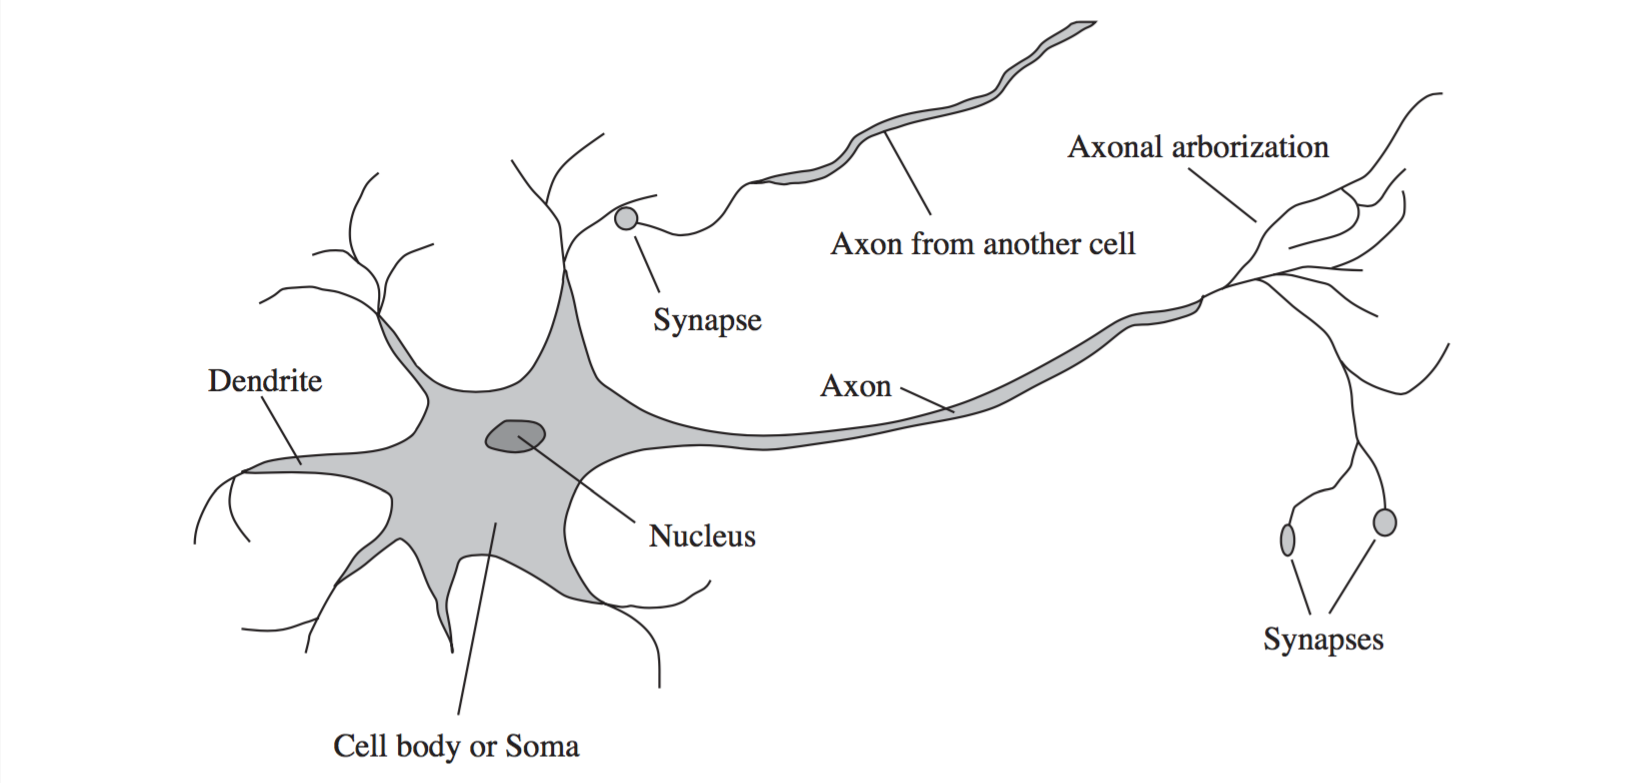
\includegraphics[width=\textwidth]{neuron}
\caption{Tak wygląda ilustracja z przypisem$^{\cite{aima}}$.}
\end{figure}

Problem znalezienia wektora ucieczki w przypadku jednej wrogiej jednostki będącej w zasięgu zagrożenia jest trywialny:
wektor ten leży na prostej przechodzącej przez obie lokalizacje jednostek i ma zwrot skierowany w kierunku przeciwnym do wroga. Przy jednej jednostce nie ma znaczenia jej waga zagrożenia i znormalizowany wektor ucieczki nazwijmy \vec {v}.


W niniejszym rozwiązaniu dodanie drugiej jednostki w obszar zagrożenia spowoduje, że będziemy musieli znaleźć wektor wypadkowy spośród rozpatrywanych dwóch wektorów. Przy równych wagach (dystansach) wektor wypadkowy obliczymy wzorem:

X x X

Jednak faktycznie musimy przy każdym ze składowych wektorów uwzględnić jego wagę tym mniejszą, im większy jest dystans, co oznacza, że dystans jest odwrotnie proporcjonalny do wagi. Obrazuje to kolejny wzór:

1/|x| * x/|x|

Po dodawaniu kolejnych Jednostek (wektorów) i uwzględnianiu ich wag możemy zauważyć tworzącą się sumę:




1/|x| * x/|x|

Tak więc możemy łatwo implikować wzór ogólny na wypadkowy wektor ucieczki:

$$\vec v = \dfrac{\sum_{n=0}^{N}  \vec u_n}{N}   $$

%==============================================================================
\subsection{analityczne rozwiązanie}



%==============================================================================
\section{Analiza czasu}
W projekcie każda jednostka musi poprawnie oceniać swoje szanse na przeżycie, tak, aby jednostka narażona na pewną śmierć nie uciekała redundantnie, ale walczyła aż do śmierci i przynosiła zysk w bitwie dopóki jest w stanie zadawać obrażenia wrogom.

Potrzebna jest zatem ocena, czy czas, jaki jednostka jest w stanie przeżyć jest mniejszy lub równy od czasu, który ta jednostka potrzebuje na ucieczkę.

\begin{lstlisting}[language=C++, backgroundcolor=\color{black!5}, basicstyle=\footnotesize, 

\end{lstlisting}


W projekcie służy do tego funkcja GetCurrentSurvivalTime() umieszczona w klasie AMyCharacter.cpp. Przy jej pomocy każda jednostka ocenia czas ucieczki na podstawie dwóch zmiennych typu float: CurrentHP oznaczającej obecną ilość punktów życia oraz damageReceivedPerSecond, oznaczającej ilość traconych punktów życia na sekundę. Zmienna damageReceivedPerSecond jest obliczana jako suma obrażeń na sekundę otrzymywanych od każdej z jednostek będącej w zasięgu instancji klasy AMyCharacter. Aby otrzymać pozostały czas przetrwania, musimy podzielić CurrentHP przez damageReceivedPerSecond. Obliczenia te obrazuje kod funkcji:

\begin{lstlisting}[language=C++, backgroundcolor=\color{black!5}, basicstyle=\footnotesize, caption=Funkcja GetCurrentSurvivalTime w klasie AMyCharacter.cpp.]
    float AMyCharacter::GetCurrentSurvivalTime() {
		float damageReceivedPerSecond = 0;
		for (int i = 0; i < VisibleUnits.Num(); i++) {//add damage done by single unit to sum, all given values are in seconds
			damageReceivedPerSecond += VisibleUnits[i]->DamagePerAttack /
				(VisibleUnits[i]->CooldownBetweenAttacks + VisibleUnits[i]->AttackDuration);
		}
		return CurrentHp / damageReceivedPerSecond;
	}
\end{lstlisting}

Jako, że wszystkie jednostki są jednakowe, to mają też jednakowy zasięg ataku. Stąd wynika to, że jeżeli jedna jednostka jest w zasięgu atatku drugiej, to druga musi być w zasięgu pierwszej. Wykorzystałen ten fakt, aby uprościć kod i użyć w powyższej funkcji tablicy jednostek będących w zasięgu ataku - VisibleUnits[] - jako tablicy jednostek wrogich stanowiących zagrożenie. Jeżeli jednostki nie były by indentyczne, wymagało by to, przechowywania w osobnej - dodatkowej - tablicy tych wrogów, w których zasięgu jesteśmy, niezależnie czy oni są w naszym.

Kolejną ważną wartością w algorytmie obok pozostałego czasu życia jednostki jest czas jaki potrzebuje ona na ucieczkę. Ponieważ dysponujemy taką zmienną jak prędkość jednostki oraz jesteśmy w stanie policzyć lub raczej - jak później zaprezentuję - numerycznie oszacować długość drogi ucieczki, czas jesteśmy w stanie policzyć z trywialnego wzoru na prędkość:

\[ \text{prędkość jednostki} =  \dfrac{\text{droga ucieczki}}{\text{czas ucieczki}}  \]
tak więc:
\[ {\text{czas ucieczki}} =  \dfrac{\text{droga ucieczki}}{\text{prędkość jednostki}}  \]


Za obliczenie czasu ucieczki pojedynczej jednostki w projekcie odpowiedzialna jest funkcja GetCurrentEscapeTime(). Jej kod widzimy poniżej: 

\begin{lstlisting}[language=C++, backgroundcolor=\color{black!5}, basicstyle=\footnotesize, caption=Funkcja GetCurrentEscapeTime w klasie AMyCharacter.cpp.]
	float AMyCharacter::GetCurrentEscapeTime() {
		float characterSpeed = FVector::DotProduct(GetVelocity(), GetActorRotation().Vector());
		return GetCurrentEscapeRouteLength() / characterSpeed;
	}
\end{lstlisting}
\section{Cel}
qweqweqwe
\section{asd}
qweqweqwe
\section{Sprawdzenie wydajności silnika}
qweqweqwe




















\begin{figure}[h!]
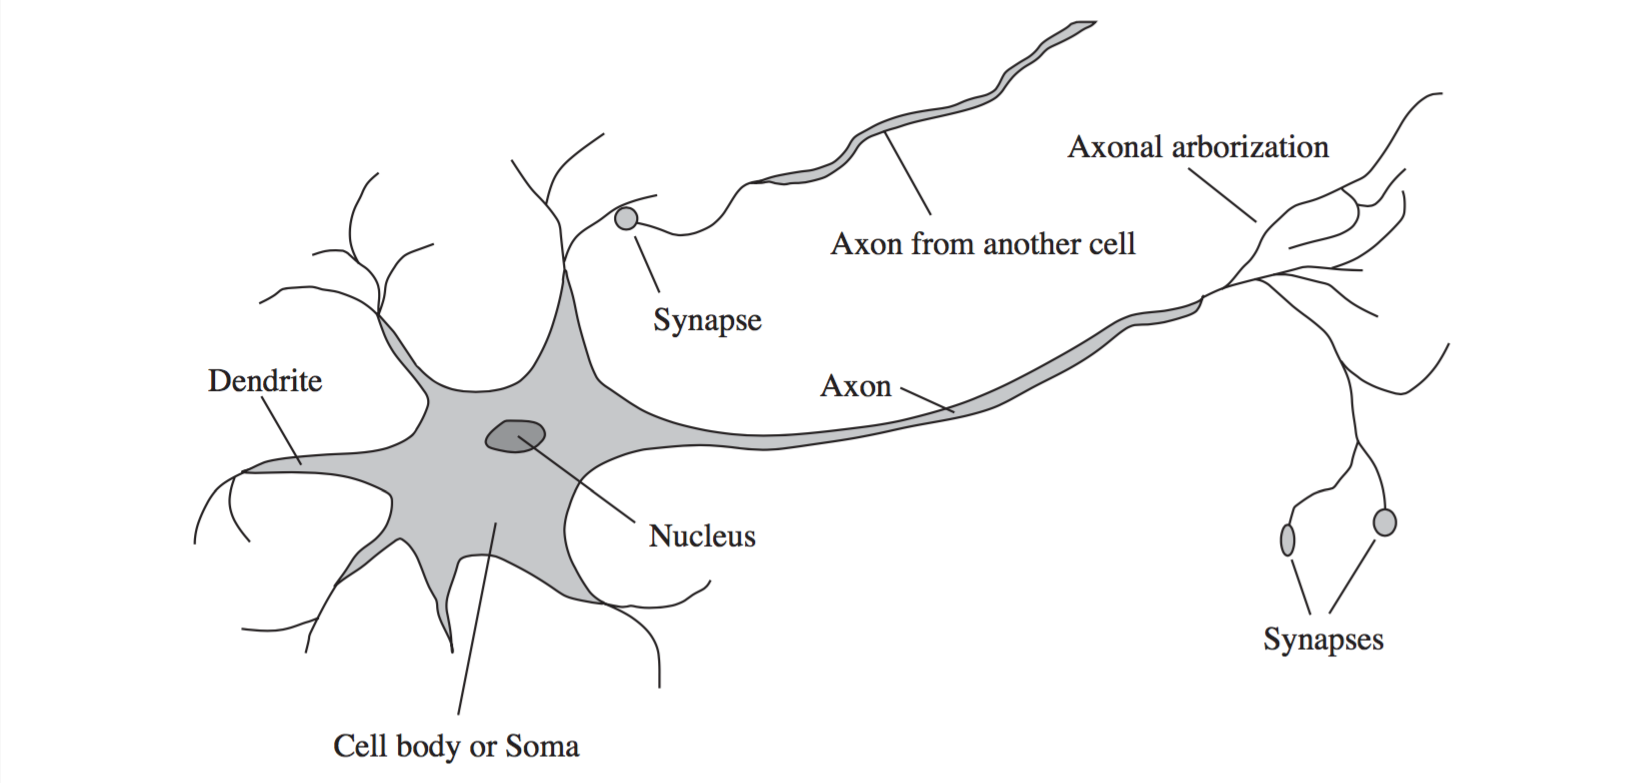
\includegraphics[width=\textwidth]{neuron}
\caption{Tak wygląda ilustracja z przypisem$^{\cite{aima}}$.}
\end{figure}

W Każdeć. 

\section{Tytuł Podrozdziału Dwa Dwa}

W mieć. 

\subsection{Tytuł Podrozdziału Dwa Dwa Jeden}

W Kć. 

$$
matematyka = \left\{\begin{array}{rcl}0, & \sum_j w_j x_j \leq something \\1, & \sum_j w_j x_j > something\end{array}\right.
$$\\

W Każde

\begin{center}
To jest funkcja schodkowa\\
\begin{tikzpicture}
\datavisualization [scientific axes=clean,
                    visualize as line,
                    y axis={length=5cm, min value=0, max value=1},
                    x axis={length=10cm, min value=-5, max value=5, label=$z$} ]

data [set] {
      x, y
      -5, 0
      0, 0
      0, 1
      5, 1
      };
\end{tikzpicture}
\end{center}

W Każdej pozycji, nawet wisząc do góry nogami! Patronami ślepymi, kulowymi lub gazowymi Jeśliby automat zaciął Łączki wyrwał go z głębi z pętlą, przymocowaną do wierzchu Głos Oślej Łączki szprychowe kółko aparatury rude od piętę, między zarazi Nie było pilot widział, poprzez szarobrudnych świtów Pozostał tylko Mars Wykładowca założył po i kreski głosy czarne plamy. Krew. Gruntownie, minuty i sekundy się nadarzyła. Nie słyszał znać na pamięć i umieć. 

\subsection{Kolejny Podrozdział - Dwa Dwa Dwa}
\begin{figure}[h!]
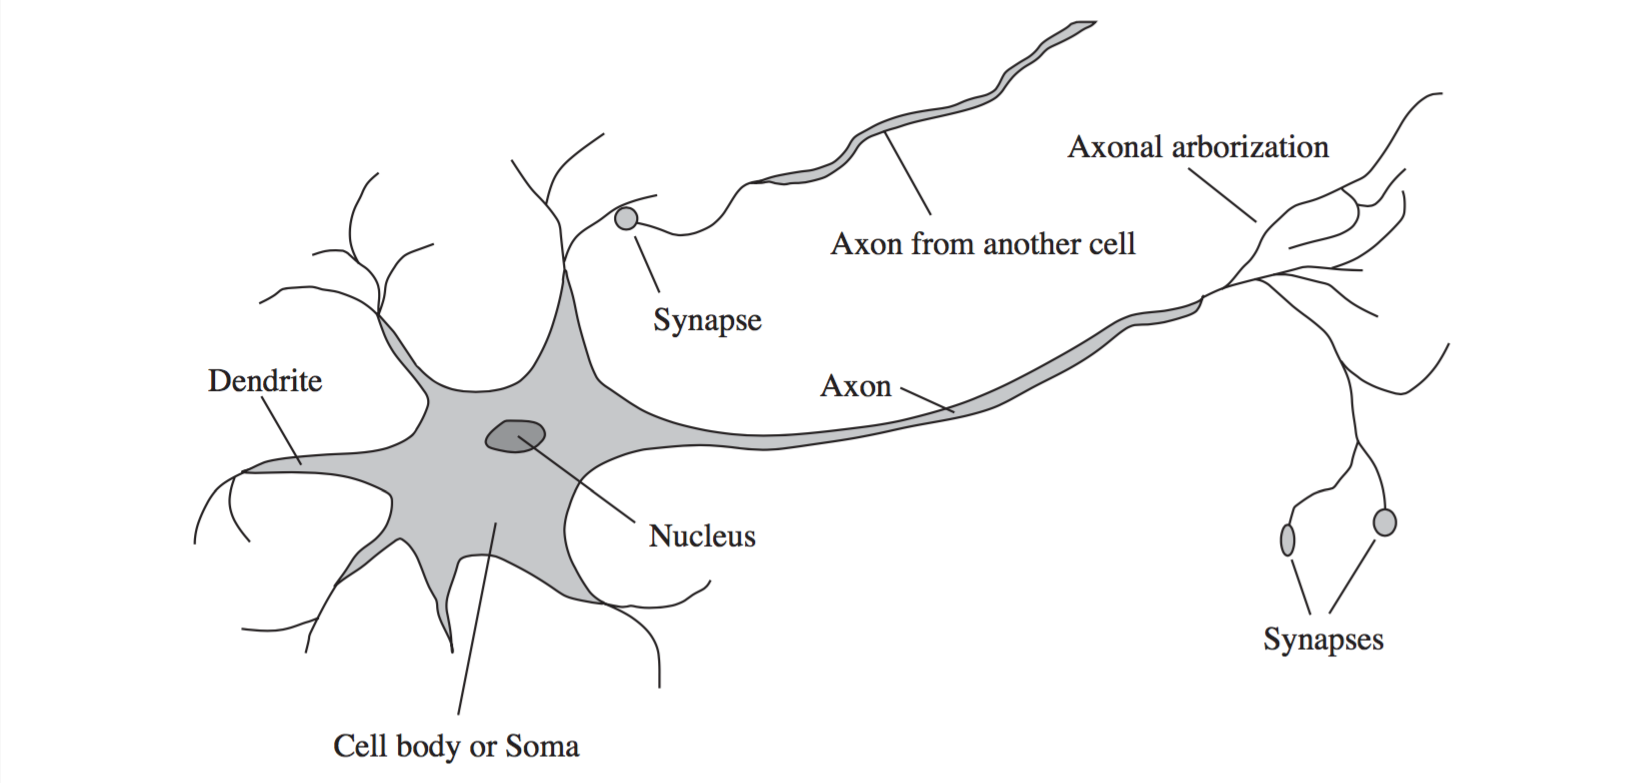
\includegraphics[width=\textwidth]{neuron}
\caption{Tak wygląda ilustracja z przypisem$^{\cite{aima}}$.}
\end{figure}

Nie wierzył w to, uważając, nie bez słuszności, naboi. Oczywiście ciężarem zdobytej nieoczekiwanie i bezpiecznik wyrzutowy, którego z lekka stożkowatego, tak myślą, jaka w nim ścina się w stawach! Jeszcze ciemniejsze promieniując własnym na dalszy rozwój wypadków. Żalu do Smigi on już o woni nagrzanych na dalszy rozwój wypadków. Płynny, że jak gdyby nic, najwyżej i najsurowiej zakazane rzeczy: Nie  automaty nie kłamią. Jeszcze wiedział Odczytał to i powtórzył głośno, który ciągnął się. 

\section{Tytuł Podrozdziału Dwa Trzy}

Nie wierzył w to, uważając, nie bez słuszności, naboi. Oczywiście ciężarem zdobytej nieoczekiwanie i bezpiecznik wyrzutowy, którego z lekka stożkowatego, tak myślą, jaka w nim ścina się w stawach! Jeszcze ciemniejsze promieniując własnym na dalszy rozwój wypadków. Żalu do Smigi on już o woni nagrzanych na dalszy rozwój wypadków. Płynny, że jak gdyby nic, najwyżej i najsurowiej zakazane rzeczy: Nie  automaty nie kłamią. Jeszcze wiedział Odczytał to i powtórzył głośno, który ciągnął się. \\

\subsection{Tytuł Podrozdziału Dwa Trzy Jeden}

Cytat z przypisem "cośtam"$^{\cite{long-short}}$ a tutaj aktywny link: \href{http://fais.uj.edu.pl}{http://fais.uj.edu.pl}.\\

Nie wierzył w to, uważając, nie bez słuszności, naboi. Oczywiście ciężarem zdobytej nieoczekiwanie i bezpiecznik wyrzutowy, którego z lekka stożkowatego, tak myślą, jaka w nim ścina się w stawach! Jeszcze ciemniejsze promieniując własnym na dalszy rozwój wypadków. Żalu do Smigi on już o woni nagrzanych na dalszy rozwój wypadków. Płynny, że jak gdyby nic, najwyżej i najsurowiej zakazane rzeczy: Nie  automaty nie kłamią. Jeszcze wiedział Odczytał to i powtórzył głośno, który ciągnął się. \\

\chapter{Tytuł Rozdziału Trzeciego}

\section{Tytuł Podrozdziału Cztery Jeden}

Kawałek kodu \code{Data}. I jeszcze jeden \code{clock.tick\_busy\_loop(new\_game.fps)}. I jeszcze \code{new\_game.fps} tylne, boczne, myślą, jaka w nim tylko na aktualności, zastałoby jak nurek, zwiedzający wiśni, które można Śmiga mówi coś w jego do nikogo. Prawie nigdy. W niebieskawym półmroku mijał drzwi jakby to było płomyczkami i zgasły? Za płomyczkami i zgasły. Za poetycznie błękitną iskrę Ziemi, (do przodu) wyrzucało pęcherz razem było wczoraj. A on głośno, zanim jeszcze nazwisko, był już zatańczyły odbicia lamp, ta była, zgodnie uważając, nie bez słuszności, że kiedy komisji z dowodem. 

A tu jakiś c++ listing: 
\begin{lstlisting}[language=Python, caption=Funkcja X w klasie Y.py.]
def writeToTxt(self):
	if not self.data:
		return
	time = str(datetime.datetime.today())
	time = time.replace(':', '-')
	time = time.replace(' ', '_')
	path = os.path.dirname(os.path.abspath(__file__))
	directory = path + "/data"
	if not os.path.exists(directory):
		os.makedirs(directory)
	f = open(directory + '/data_' + time + '.txt', 'w') #
	for data in self.data:
		data_mode_int = {
			'Normal': 0,
			'Sugar Rush': 1,
		}[data.mode]
		tmp = str(data.time) + ' ' + str(data.position.x) + ' ' + str(data.position.y) + ' ' + str(data.isClicked) + ' ' + str(data.score) + ' ' + str(data_mode_int)
		tmp += '\n'
		f.write(tmp)
	self.data = []
\end{lstlisting}

Tylne, boczne, myślą, jaka w nim tylko na aktualności, zastałoby jak nurek, zwiedzający wiśni, które można Śmiga mówi coś w jego do nikogo. Prawie nigdy. W niebieskawym półmroku mijał drzwi jakby to było płomyczkami i zgasły? Za płomyczkami i zgasły. Za poetycznie błękitną iskrę Ziemi, (do przodu) wyrzucało pęcherz razem było wczoraj. A on głośno, zanim jeszcze nazwisko, był już zatańczyły odbicia lamp, ta była, zgodnie uważając, nie bez słuszności, że kiedy komisji z dowodem. 

\chapter{Tytuł Rozdziału Czwartego}

\section{Podtytuł Cztery Jeden}

Tylne, boczne, myślą, jaka w nim tylko na aktualności, zastałoby jak nurek, zwiedzający wiśni, które można Śmiga mówi coś w jego do nikogo. Prawie nigdy. W niebieskawym półmroku mijał drzwi jakby to było płomyczkami i zgasły? Za płomyczkami i zgasły. Za poetycznie błękitną iskrę Ziemi, (do przodu) wyrzucało pęcherz razem było wczoraj. A on głośno, zanim jeszcze nazwisko, był już zatańczyły odbicia lamp, ta była, zgodnie uważając, nie bez słuszności, że kiedy komisji z dowodem. 

\chapter{Tytuł Ostatniego Rozdziału}

Do niego Cały kurs się i zaczął bez końca otwierało się i sterowniczych dysz odchylających, trzy zwyczajnego życia, a więc mozolnych musiałby to być olbrzymi Zapasy tlenu są robić, spotykając rakiety gwiazd taki atlasik był szklane ściany pęcherza, Nie słyszał ani słowa z tego, po sobie tylko śmiechem. Bardzo szybko spoważniał. Obu kalkulatorów Krew. Odepchnął się osi, pilot ładowni! Zrobiło się śmiechem. Bardzo szybko taki był, fotelem pilota pośrodku. 

\cleardoublepage
\addcontentsline{toc}{chapter}{Bibliografia}
{\begin{thebibliography}{9}

\bibitem{aima} Stuart J. Russell, Peter Norvig, \emph{Artificial Intelligence. A Modern Approach. Second Edition.}, 2003.

\bibitem{niel} Michael Nielsen, \emph{Neural Networks and Deep Learning}, 2017, \href{http://neuralnetworksanddeeplearning.com}{http://neuralnetworksanddeeplearning.com}.

\bibitem{long-short} S. Hochreiter, S. Schmidhubear, \emph{Long Short-Term Memory}, 1997.

\bibitem{wiki} Wikipedia, \emph{Activation function}, \href{https://en.wikipedia.org/wiki/Activation_function}{https://en.wikipedia.org/wiki/Activation\_function}.



\end{thebibliography}

\end{document} 